
\clearpage

\section{Una revisión al ADN}
\label{sec:ADN}
La importancia de este capitulo es dar las bases necesarias para ADN


\subsection{Historia del ADN}
La epopeya del ADN tiene sus inicios en 1869 con un bioquímico llamado Friedrich Miescher, esté estaba interesado en la estructura química de las fascinantes unidades fundamentales de la vida conocidas como células.
Miescher viajaba todos los días a la clínica más cercana para tomar las vendas sucias, esto debido a que estaban recubiertas de pus (lo cual era una buena fuente de leucocitos), añadiendo álcali hizo que los núcleos se abrieran liberando sus componentes, de esta manera Miescher extrajo un componente(ADN), al que el nombro nucleína, realizando un análisis de esta nucleína mostró que era un ácido que contenía fósforo y por tanto no calificaba en en ninguno de los grupos conocidos en ese momento como carbohidratos y proteínas, este fue clasificado como un ácido nucleico y su relevancia biológica no fue descubierta hasta mucho tiempo después \cite{Susan}.\\

En 1928 Fredrick Griffith realizaba una investigación con neumococos, tenia dos tipos: el primero patógeno  fue cultivado en placas de petri conocido como s(smooth-suave) debido a su apariencia, el segundo inofensivo y conocido como r(rough-áspero), Griffith descubrio que al añadir un extracto de los neumococos tipos S al tipo R, esté ultimo podría heredar las propiedades del tipo S, este -principio de transformación- indicaba que el extracto contenía la molécula de herencia.\\

Oswald Avery junto con MacLeod y McCarty demostrarón que substancia efectiva en el experimento de Griffiths era la molecula de ADN y que a su vez, era el portador de genes en la célula, también es importante mencionar que Alfred Hershey y Martha Chase quienes confirmaron la conclusión en 1952 mediante experimentos con trazadores radioactivos\cite{Thormod}.\\

Es relevante mencionar otros aportes significativos: \\
1.Erwin Chargaff encontro una regularidad peculiar en los radios de las bases de los nucleotidos.\\
2.Sven Furger trabajo en la estructura de los componentes del ADN, encontró que la base plana(plano de la citocina) era perpendicular a la molecula de azucar.\\
3.Rosalind Franklin logro distinguir dos tipos de ADN dependiendo de la hidratación y que ambos tenían estructura helicoidal mediante cristalográfia, véase figura ~\ref{fig:rf}.

\begin{figure}[htbp]
    \centering
    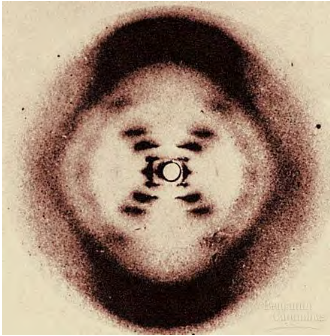
\includegraphics[width=0.5\linewidth]{./Figures/RF.png}
    \caption[Fotografía cristalográfica del ADN]{Fotografiá cristalográfica del ADN tomada por Rosalind Franklin en 1952}
    \label{fig:rf}
\end{figure}
El ultimo paso hacia la estructura del ADN fue llevado acabo por James Watson y Francis Crick en el laboratorio de Cavendish en francia, juntos trabajarón en diferentes modelos de la molecula de ADN , en 1953 publicarón un articulo en la prestigiosa revista Nature titulado: "Molecular Structure of Nucleid Acids", el articulo solo tenia una pagina, pero era de un impacto significativo debido al modelo de ADN que contenía, un modelo de doble hélice(figura ~\ref{fig:jw}), y sugerían que el emparejamiento  especifico que habían postulado intuía un posible mecanismo para copiar material genético.
\begin{figure}[htbp]
    \centering
    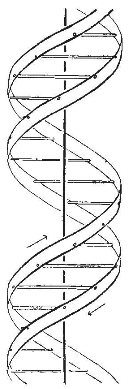
\includegraphics[width=0.15\linewidth]{./Figures/DNA1.png}
    \caption[Diagrama esquemático del ADN]{Diagrama esquemático del ADN publicado por Watson y Crick en 1953, imagen tomada de \cite{jwfc}.}
    \label{fig:jw}
\end{figure}
\subsection{Estructura del ADN}
El ADN es una molécula compuesta por seis diferentes tipos de bloques: cuatro bases, citocina, timina, guanina, adenina, junto con una molécula de azúcar y un grupo fosfato, el fosfato el azucar y la base forman un nucleotido, y el ADN esta conformado por dos cadenas largas de nucleotidos, si todo el ADN de solo una celula humana fuera unido y alargado, seria aproximadamente de dos metros de largo
If all the DNA in a single human cell was tied together and stretched out, it would be approximately 2 meters long. One strand of DNA binds to the other strand through hydrogen bonds that extend between base pairs. Thus, C binds specifically with G and A binds with T forming the C – G and A – T base pairs.mkqkjjkjsfdsfdsfd
The human double helix contains about 6 billion base pairs. Three adjacent bases (a triplet or codon) on one strand code for a certain amino acid in a protein. If a protein consists of 200 amino acids, the DNA that codes for this protein consists of at least 600 bases, i.e., 200 triplet codons. This is a gene.

\subsubsection{Daño inducido por radiación al ADN}
The most important types of damage to the DNA molecule, induced by radiation, are outlined in the figure below. There are four common types of damage
\paragraph{Rompimientos simples}
A single strand break is simply a break in one of the sugar-phosphate chains. This damage is usually simple to repair and, in experiments, it has been shown that approximately 90\% of the single strand breaks are repaired in the course of one hour at 37o
C. 2.
\paragraph{Rompimientos dobles}
This type of damage involves both strands of the DNA helix, which are broken opposite to each other or within a distance of a few base pairs. This type of damage (also called a clustered damage) would kill the cell and in experiments with bacteria a correlation is found between double strand breaks and cell death (David Freifelder in the 1960-ties).
Double strand breaks are more difficult to repair correctly. However, they actually are. The DNA-molecule is packed together with proteins supporting the structure and preventing the pieces from falling apart, even when breaks occur on both strands of the helix. There are in fact a number of mechanisms that complex organisms (such as humans) have evolved for repairing double strand breaks. But as one might guess, this type of break is more difficult to repair and does correlate with cell death and observable damage to chromosomes.
3.
\paragraph{Daño base}
Experiments indicate that the radiation sensitivity varies from one base to another. After an initial ionization, rapid electronic reorganizations take place with the result that the damage is transported to certain regions of the macromolecule. The base guanine is particularly sensitive.
Damage to a base is one of the starting points for a mutation. If a base is changed, information may be lost or changed. As the result of a misrepair or no repair, the altered triplet codon is likely to lead to insertion of the incorrect amino acid in the pro- tein. In turn, the changed protein might not function properly.
\paragraph{Dimeridos de pirimidina}
Pyrimidine dimers are also examples of clustered damage. In this example, two adjacent bases, T and T, on the same strand have been chemically altered.
This is but one out of a
myriad of possibilities. All the possibilities have the common feature that two or more damaged sites lie in close proximity to one another.
Double strand break
Base damage
We shall return to repair mechanisms, but would like to mention the problems posed by clustered damage. One of the strands is needed to replicate the adjacent strand. When both strands are damaged at the same site there is no template to work from. This is in contrast to damage such as a single base alteration or a single strand break
\subsection{Daño Celular}
\subsubsection{Reparación del ADN}
\subsubsection{Mecanismos de defensa}
\subsubsection{Respuesta adaptativa}
\subsubsection{Effects of ionizing radiation in nonirradiated cells}
\cite{willmari}
